\documentclass[10pt]{article}
\usepackage[a4paper,margin=1cm,landscape]{geometry}
\usepackage[utf8]{inputenc}
\usepackage[french]{babel}
\usepackage{libertine}
\usepackage[T1]{fontenc}
\usepackage{xcolor}
\usepackage{tikz}
\usepackage{graphicx}

\title{Modèle <<Squad\footnote{Le  terme <<squad>> (traduit  ici par <<équipe>>) est le  mot utilisé  par Spotify pour  une équipe  de  développement petite, cross-fonctionnelle et  auto-organisée.}
  Health Check>> - Version française {\small basé  sur la  version 1 de  septembre 2014}}
\date{}

\begin{document}

\maketitle

\begin{tikzpicture}[remember picture, overlay]
  \node [shift={(-100 mm,-70 mm)}]  at (current page.north east) {
    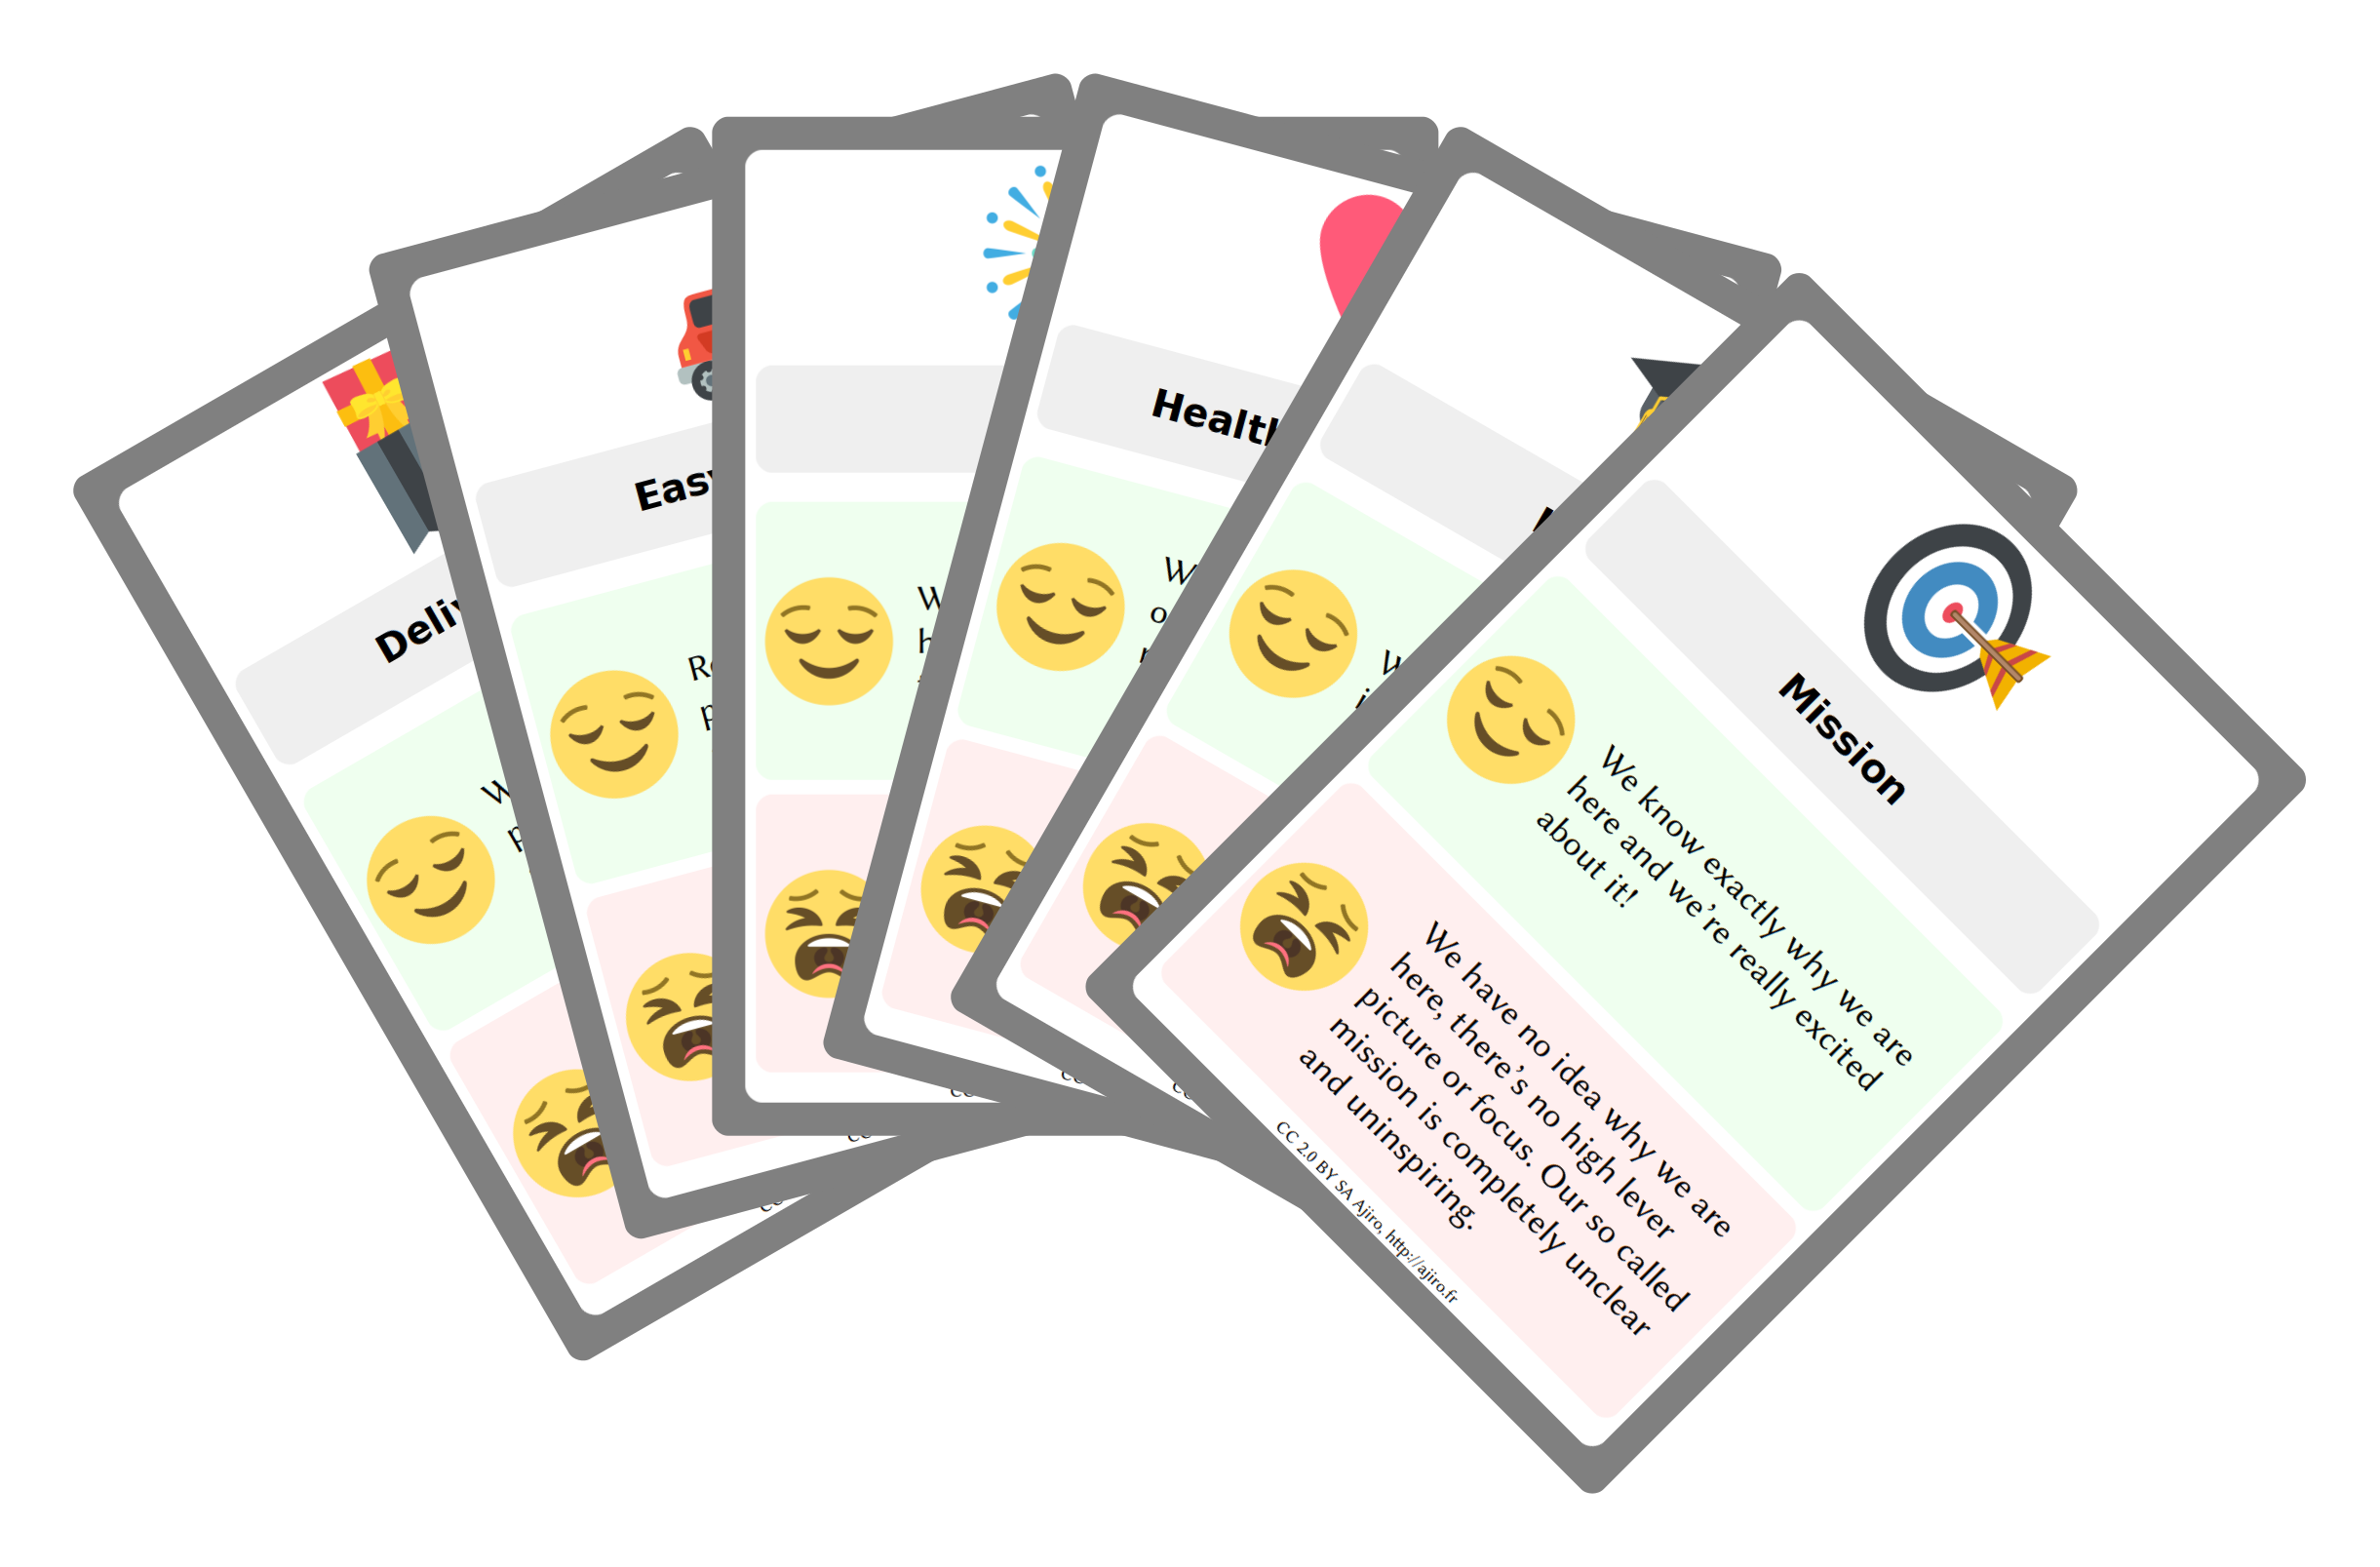
\includegraphics[width=6cm]{includes/hand}
  };
\end{tikzpicture}

\begin{tikzpicture}[remember picture, overlay]
  \node [shift={(-40 mm,-80 mm)}]  at (current page.north east) {
    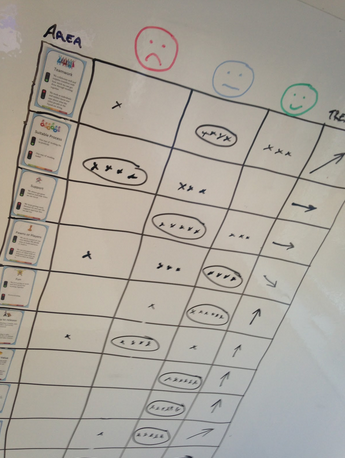
\includegraphics[width=5cm]{includes/equipe}
  };
\end{tikzpicture}

\begin{tikzpicture}[remember picture, overlay]
  \node [shift={(-54 mm,-145 mm)}]  at (current page.north east) {
    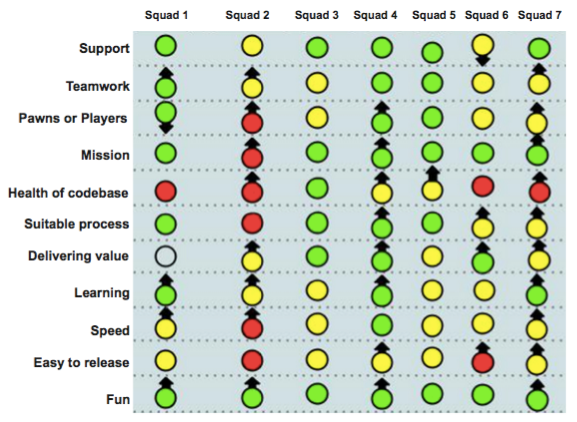
\includegraphics[width=8cm]{includes/evolution}
  };
\end{tikzpicture}

\begin{minipage}{0.6\linewidth}
\section*{De  quoi  s’agit-il ?}
Un  atelier et  une technique de  visualisation  aidant  les équipes à s’améliorer.

\section*{Audience  ?}
\begin{itemize}
  \item L’équipe  elle-même 
  \item Les personnes apportant leur  support à l’équipe
  \item (managers,  coachs, etc.) 
\end{itemize}


\section*{Comment utiliser  ce  modèle}
\begin{itemize}
  \item Avec un jeux de carte
  \item Rassemblez  tous  les membres de  l’équipe  dans  la  même  salle 
  \item Discutez  sur les cartes  de  questions. Chacune d’entre elle  est un  indicateur  de  bonne santé,  accompagné  d’un  exemple de  très  bonne performance et  d’un  exemple particulièrement  inefficace. 
  \item Demander  à l’équipe  comment elle  se  positionne sur chacun  de  ces indicateurs,  en  utilisant une méthode favorisant  les décisions de  groupe  (par  exemple : avec  les cartes  de  vote).  
  \item Discutez  les tendances d’évolution de  ces indicateurs (la situation s’améliore-t-elle ? Est- elle  stable  ou  se  dégrade-t-elle  ?)
  \item Matérialisez  visuellement  les résultats de  ces discussions.  
  \item Utilisez des données quantitatives (estimation,  mesures,  extrapolation...)  pour  aider l’équipe  à s’améliorer.  
\end{itemize}


\section*{Idées de  mises en  œuvre}
  Les cartes  sont  uniquement  un  point de  départ  pour  initialiser des conversations produc:ves. L’équipe  doit  se  sen:r libre d’ajouter/ôter/modifier toute ques:on afin  de  correspondre  à ce  qu’elle considère comme important pour  elle.

  Assurez-vous  que cet outil  soit  utilisé  en  support de  l’équipe  dans  son amélioration  et  surtout pas pour  l’évaluer!
\end{minipage} \hfill

\begin{tikzpicture}[remember picture, overlay]
  \node [shift={(-58 mm,-19 cm)}]  at (current page.north east) {
    \noindent\fcolorbox{lightgray}{lightgray}{
      \begin{minipage}{9 cm}
        \section*{\normalsize Crédits}
        \scriptsize
        \begin{itemize}
          \item Modèle  Health  check : Henrik  Kniberg \& Kristian  Lindwall,
          \item avec  l’aide  des autres  coaches agiles  chez  Spotify
          \item Design  graphique des cartes: Martin  Österberg
          \item Traduc:on française : Thomas  Clavier,  Séverin Legras, Hervé Taboucou, avec  l’aide  des membres d'Ajiro.fr
        \end{itemize}
        Distribuez, modifiez, réutilisez  ces contenus  sous  licence CC~BY-SA~3.0~FR
      \end{minipage}
    }
  };
\end{tikzpicture}
  

\end{document}
